\documentclass[14pt]{article}

\usepackage[russian]{babel}
\usepackage[utf8]{inputenc}
\usepackage{amsmath,amssymb}
\usepackage{parskip}
\usepackage{caption}
\usepackage{textcomp}
\usepackage{gensymb}
\usepackage[dvips]{graphicx}
\usepackage{wrapfig}
\usepackage{color}
\usepackage{setspace}
%\usepackage{hyperref}
\usepackage{epstopdf}

\oddsidemargin=0 cm
\evensidemargin=0 cm
\textwidth=170 mm
\textheight=230 mm
\topmargin=0 cm
\voffset= -2cm
\pagenumbering{false}
\newlength{\varheight}
\setlength{\varheight}{3.1cm}
\setlength{\parindent}{0cm}
\spacing{1.1}
\parskip=2mm
\clubpenalty=10000
\widowpenalty=10000
\captionsetup[figure]{labelformat=empty}

\begin{document}

\begin{center}
\Large{\textbf{Силы трения}}

\textbf{15.04.2017}
\end{center}
\vspace{5mm}

1. Тело массой $m$ лежит на наклонной плоскости с углом наклона $\alpha$, коэффициент трения между телом и плоскостью $\mu$.

а) При каком минимальном $\alpha_0$ тело начнет движение?

б) Найдите ускорение тела при $\alpha>\alpha_0$.

Пусть теперь тело тянут вверх вдоль наклонной плоскости с постоянной силой.

в) Какой минимальной силы $F_1$ достаточно, чтобы не давать телу соскальзывать вниз?

г) Какова минимальная сила $F_2$, при которой тело начинает двигаться вверх?

Пусть теперь можно прикладывать силу под произвольным углом $\beta$ к горизонту. Необходимо добиться того, чтобы тело двигалось вверх вдоль плоскости.

д) Чему равна минимальная необходимая сила $F_0$ и под каким углом $\beta_0$ она должна быть направлена?

\begin{figure}[h]
\begin{center}
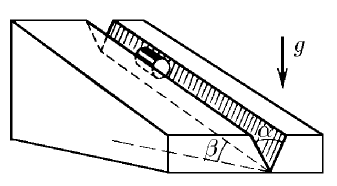
\includegraphics[width=0.28\textwidth]{friction1.png}
\hspace{1cm}
\includegraphics[width=0.13\textwidth]{friction2.png}
\hspace{1cm}
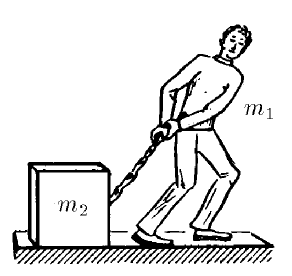
\includegraphics[width=0.23\textwidth]{friction3.png}
\caption{\hspace{0.5cm}К задаче 2\hspace{3cm}К задаче 3\hspace{2.5cm}К задаче 4}
\end{center}
\end{figure}

2. Цилиндр скользит по желобу, имеющему вид двугранного угла с раствором $\alpha$ (рис). Ребро двугранного угла наклонено под углом $\beta$ к горизонту. Плоскости двугранного угла образуют одинаковые углы с горизонтом. Коэффициент трения между цилиндром и поверхностью желоба $\mu$. Определите ускорение цилиндра.

3. Нить, перекинутая через блок с неподвижной осью, пропущена через щель (рис). На концах нити подвешены грузы, масса которых $m_1$ и $m_2>m_1$. Определите ускорения грузов, если при движении нити на нее сос тороны щели действует постоянная сила трения $F$.

4. Человек массы $m_1$, оставаясь на месте, тянет за веревку груз массы $m_2$ (рис). Коэффициент трения человека и груза о горизонтальную поверхность равен $\mu$. При какой наименьшей силе натяжения веревки груз стронется с места? Под каким углом должна быть направлена веревка?

5. Сани массой $M$ движутся по ровной горизонтальной поверхности со скоростью $v_0$. На сани вертикально падает тело массой $m$, брошенное с высоты $h$. Коэффициент трения между санями и поверхностью $\mu$. Найдите скорость саней непосредственно после падения тела, а также путь, который сани проедут до остановки. С какой высоты необходимо уронить тело, чтобы сани остановились сразу после его падения?

6. Сани массой $M$ стоят неподвижно на ровной горизонтальной поверхности с коэффициентом трения $\mu$. На сани сзади запрыгивает собака массы $m$ со скоростью $v_0$, направленной вниз под углом $\alpha$ к горизонту.

а) Каким должен быть максимальный угол $\alpha_0$, чтобы сани тронулись после падения собаки?

б) Найдите путь, который проедут сани до остановки, если $\alpha<\alpha_0$.

7. Монета лежит неподвижно на наклонной плоскости с углом наклона $\alpha$, коэффициент трения между монетой и плоскостью $\mu=\tan\alpha$. Монете придали горизонтальную скорость $v$. Найдите установившуюся скорость монеты.

\begin{figure}[h]
\begin{center}
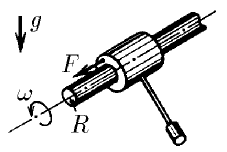
\includegraphics[width=0.18\textwidth]{friction4.png}
\hspace{1cm}
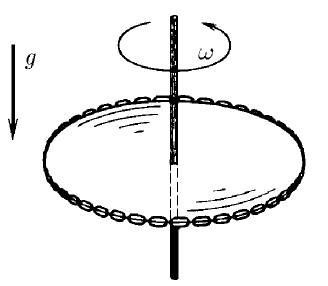
\includegraphics[width=0.25\textwidth]{friction5.png}
\hspace{1cm}
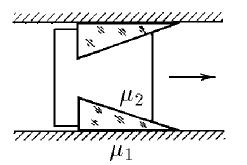
\includegraphics[width=0.23\textwidth]{friction6.png}
\caption{\hspace{-0.3cm}К задаче 8\hspace{3.2cm}К задаче 9\hspace{3.5cm}К задаче 10}
\end{center}
\end{figure}

8. Горизонтальную ось радиуса $R$, вращающуюся с угловой скоростью $\omega$, обжимает втулка с противовесом (см. рис, противовес нужен для того, чтобы втулка не вращалась). Максимальная сила трения втулки об ось $F_0$. Определите установившуюся скорость втулки под действием силы $F<F_0$, направленной вдоль оси.

9. Однородная кольцевая цепочка массы $m$ надета на горизонтальный диск радиуса $R$. Сила натяжения цепочки $T$, коэффициент трения между цепочкой и диском $\mu$. Найдите, при какой минимальной угловой скорости диска цепочка спадет с него.

10. Тело с установленными в его вырезах клиньями расположено между двумя его параллельными стенками так, как показано на рисунке. Найдите предельный угол при вершине клиньев, при котором тело может двигаться вправо и не может двигаться влево. Коэффициенты трения клиньев о стенки и тело равны $\mu_1$ и $\mu_2$ соответственно.

\begin{figure}[h]
\begin{center}
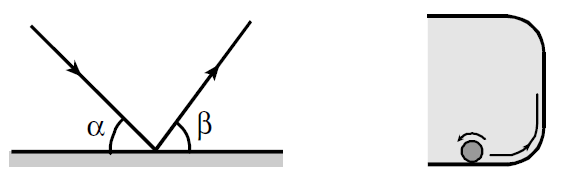
\includegraphics[width=0.45\textwidth]{friction7.png}
\hspace{1cm}
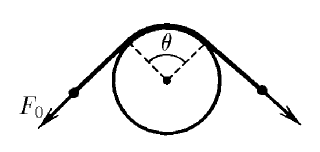
\includegraphics[width=0.3\textwidth]{friction8.png}
\caption{\hspace{-0.3cm}К задаче 11\hspace{2.8cm}К задаче 12\hspace{3.3cm}К задаче 13}
\end{center}
\end{figure}

11. Быстро вращающийся шар налетает на стену со скоростью $v_0=5$ м/с под углом $\alpha=45$\textdegree\;и отскакивает от нее под углом $\beta$ (см. рисунок). Какова скорость $v$ шара после удара, если коэффициент трения между шаром и стеной $\mu=0.3$? Рассмотрите 2 случая: $\beta=60$\textdegree\,и $\beta=30$\textdegree.

12. Быстро вращающаяся шайба скользит вдоль бортика хоккейной площадки (рис). Коэффициент трения шайбы о бортик $\mu=0.3$, трение о лед пренебрежимо мало. Во сколько раз уменьшится скорость шайбы после прохождения угла?

13. За один конец легкой веревки, охватывающей столб по дуге с углом $\theta$, тянут с силой $F_0$. Какую минимальную силу нужно приложить ко второму концу веревки, чтобы его удержать, если коэффициент трения веревки о столб равен $\mu$?

14. Через неподвижное горизонтально закрепленное бревно переброшена веревка. Чтобы удерживать груз массы $m=18$ кг, подвешенный на этой веревке, необходимо тянуть второй конец веревки с минимальной силой $F_1=120$ Н. С какой минимальной силой $F_2$ надо тянуть веревку, чтобы груз начал подниматься?

\end{document} 